%%%%%%%%%%%%%%%%%%%%%%%%%%%%%%%%%%%%%%%%%
% Beamer Presentation
% LaTeX Template
% Version 1.0 (10/11/12)
%
% This template has been downloaded from:
% http://www.LaTeXTemplates.com
%
% License:
% CC BY-NC-SA 3.0 (http://creativecommons.org/licenses/by-nc-sa/3.0/)
%
%%%%%%%%%%%%%%%%%%%%%%%%%%%%%%%%%%%%%%%%%

%----------------------------------------------------------------------------------------
%	PACKAGES AND THEMES
%----------------------------------------------------------------------------------------

\documentclass{beamer}

\mode<presentation> {

% The Beamer class comes with a number of default slide themes
% which change the colors and layouts of slides. Below this is a list
% of all the themes, uncomment each in turn to see what they look like.

%\usetheme{default}
%\usetheme{AnnArbor}
%\usetheme{Antibes}
%\usetheme{Bergen}
%\usetheme{Berkeley} %with Outline
%\usetheme{Berlin}
%\usetheme{Boadilla}
\usetheme{CambridgeUS} %This is well-looking
%\usetheme{Copenhagen}
%\usetheme{Darmstadt}
%\usetheme{Dresden}
%\usetheme{Frankfurt}
%\usetheme{Goettingen}
%\usetheme{Hannover}
%\usetheme{Ilmenau}
%\usetheme{JuanLesPins}
%\usetheme{Luebeck}
%\usetheme{Madrid}
%\usetheme{Malmoe}
%\usetheme{Marburg}
%\usetheme{Montpellier}
%\usetheme{PaloAlto}
%\usetheme{Pittsburgh}
%\usetheme{Rochester}
%\usetheme{Singapore}
%\usetheme{Szeged}
%\usetheme{Warsaw}

% As well as themes, the Beamer class has a number of color themes
% for any slide theme. Uncomment each of these in turn to see how it
% changes the colors of your current slide theme.

%\usecolortheme{albatross}
%\usecolortheme{beaver}
%\usecolortheme{beetle}
%\usecolortheme{crane}
\usecolortheme{dolphin}
%\usecolortheme{dove}
%\usecolortheme{fly}
%\usecolortheme{lily}
%\usecolortheme{orchid}
%\usecolortheme{rose}
%\usecolortheme{seagull}
%\usecolortheme{seahorse}
%\usecolortheme{whale}
%\usecolortheme{wolverine}

%\setbeamertemplate{footline} % To remove the footer line in all slides uncomment this line
%\setbeamertemplate{footline}[page number] % To replace the footer line in all slides with a simple slide count uncomment this line

%\setbeamertemplate{navigation symbols}{} % To remove the navigation symbols from the bottom of all slides uncomment this line
}

\usepackage{graphicx} % Allows including images
\usepackage{booktabs} % Allows the use of \toprule, \midrule and \bottomrule in tables
\usepackage{amsmath, amssymb, amsfonts}
\usepackage{mathrsfs}
\usepackage{amsthm}
%----------------------------------------------------------------------------------------
%	TITLE PAGE
%----------------------------------------------------------------------------------------

\title[VE216]{VE216 Recitation Class 10} % The short title appears at the bottom of every slide, the full title is only on the title page

\author{ZHU Yilun} % Your name
\institute[SJTU] % Your institution as it will appear on the bottom of every slide, may be shorthand to save space
{
UM-SJTU Joint Institute \\ % Your institution for the title page
\medskip
\textit{VE216 SU20 TA Group} % Your email address
}
\date{2020 Summer} % Date, can be changed to a custom date e.g.:\today

\begin{document}

\begin{frame}
\titlepage % Print the title page as the first slide
\end{frame}

\begin{frame}
\frametitle{Overview} % Table of contents slide, comment this block out to remove it
\tableofcontents % Throughout your presentation, if you choose to use \section{} and \subsection{} commands, these will automatically be printed on this slide as an overview of your presentation
\end{frame}

%----------------------------------------------------------------------------------------
%	PRESENTATION SLIDES
%----------------------------------------------------------------------------------------


%---------------------------------------------------
\section{Chapter 9: Laplace Transform}

\subsection{Definition}
\begin{frame}
    \frametitle{Laplace Transform}
    \begin{itemize}
        \item $s = \sigma + j \omega, e^{st} = e^{\sigma t} \cdot e^{j \omega t}$: decaying/growing term and periodic term
        \item LT Definition: 
        \[ X(s) = \int_{- \infty}^{\infty} x(t) e^{-st} dt \]
        Notice: ROC \\
        Study system behavior
        \item Compare with FT:  \[ X(j \omega) = \int_{- \infty}^{\infty} x(t) e^{-j \omega t} dt \] \\
        decompose signals; system as filters
    \end{itemize}
\end{frame}

\begin{frame}
    \frametitle{ROC}
    Definition: the subset of $\mathbb{C}$ that $X(s) = \int_{- \infty}^{\infty} x(t) e^{-st} dt < \infty$  \newline
    Consider:
    \[ X(s) = \frac{1}{(s+1)(s+2)}\]
    \begin{figure}
        
        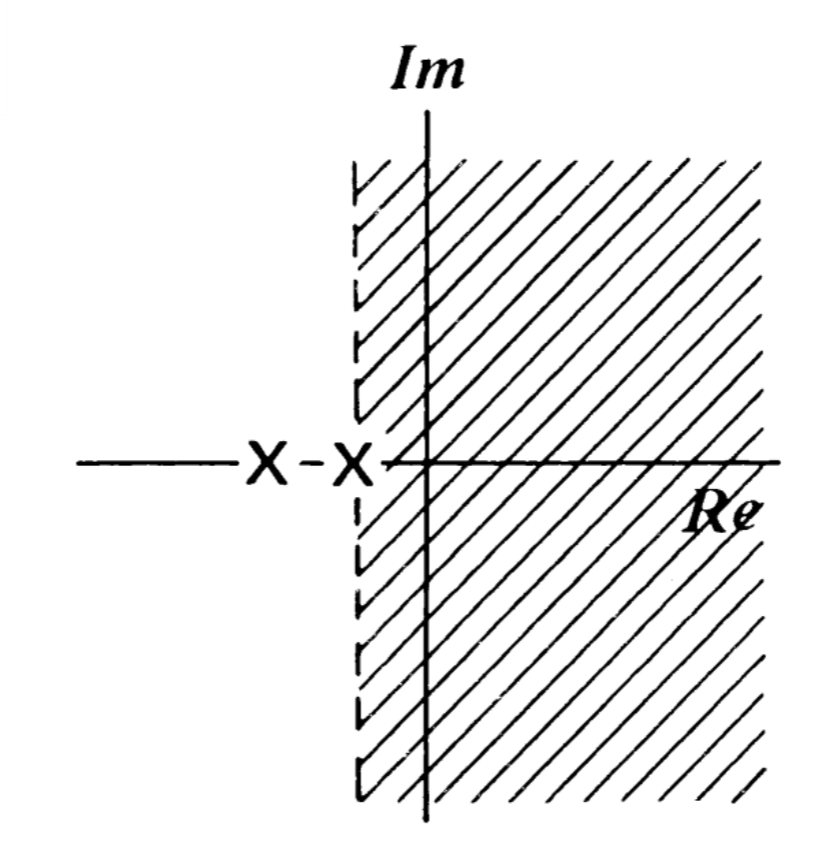
\includegraphics[width=0.3\linewidth]{roc1}
        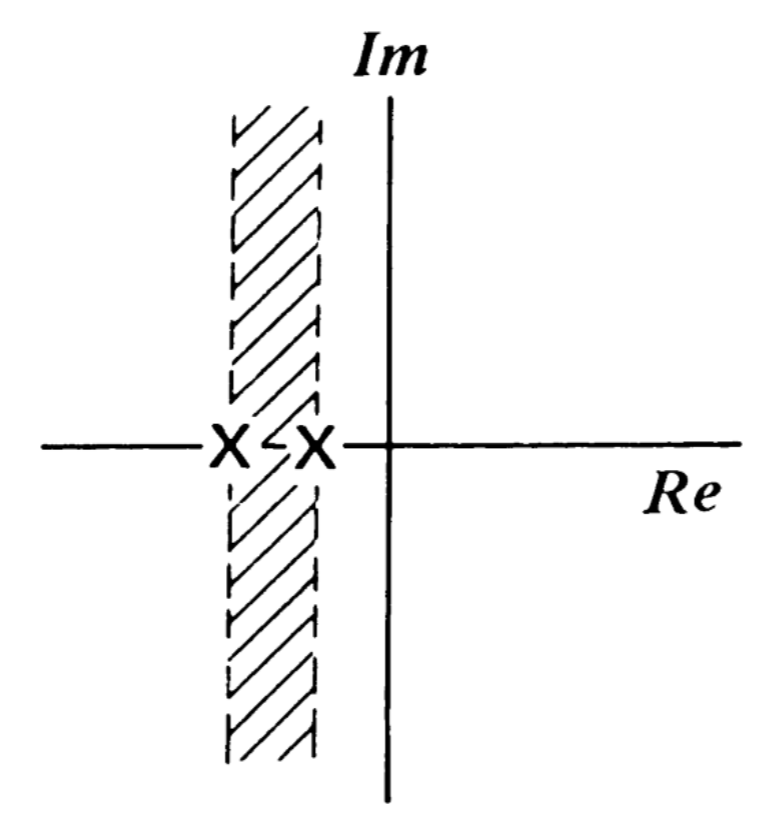
\includegraphics[width=0.3\linewidth]{roc2}
        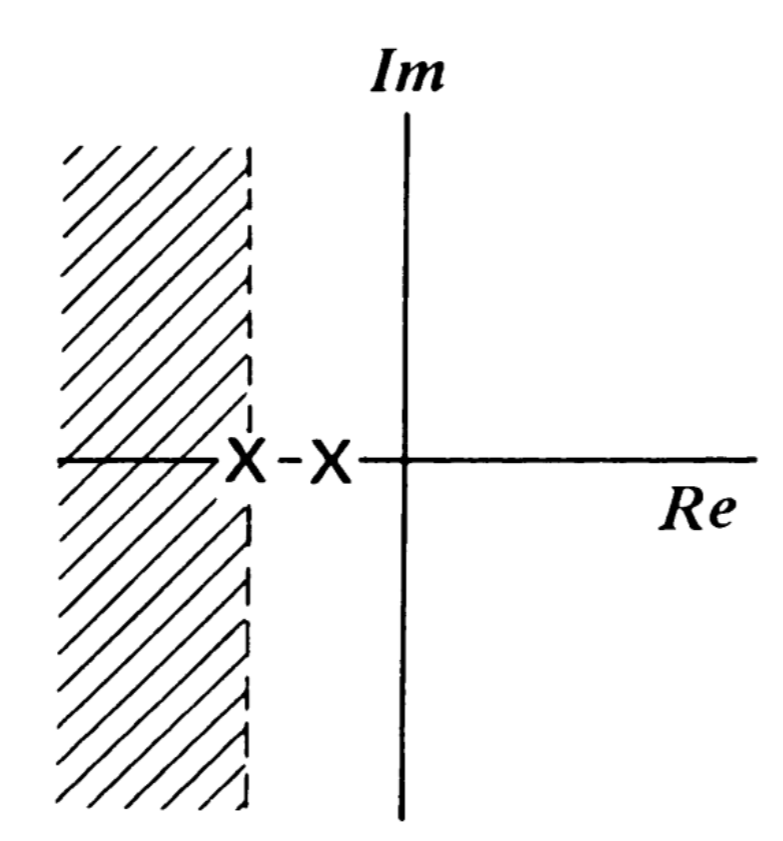
\includegraphics[width=0.3\linewidth]{roc3}
        
    \end{figure}
    Different choice of ROC corresponds to different $x(t)$. - Quiz9 \newline
    (here, $x(t)$ can be input/output signal, or the impulse response)        
\end{frame}

\subsection{Study System Behavior}
\begin{frame}
    \frametitle{LT - Study (rational) LTI System Behavior $H(s)$ }
    \begin{itemize}
        \item stable $\Longleftrightarrow$ ROC includes $j\omega$ axis
        \item casual $\Longleftrightarrow$ ROC RHP
        \item casual and stable $\Longleftrightarrow$ all poles in the left half of s-plane
        \item Not stable if: $H(s) = \frac{s^2+s+1}{s+1}$
        \item Differentiation: solve systems defined by diff. eqn. \[ \frac{d^n}{dt^n} x(t) \stackrel{\mathscr{L}}{\longleftrightarrow} s^n X(s) \]
        \item Convolution: get output y(t) \[h(t)* x(t) \stackrel{\mathscr{L}}{\longleftrightarrow} H(s) X(s)    \]
        \item Block diagram: be able to read as well as draw - Quiz10
    \end{itemize}
\end{frame}

\subsection{Exercise}

\begin{frame}[t]
    \frametitle{Exercise: HW6 Q5}
    \begin{figure}
        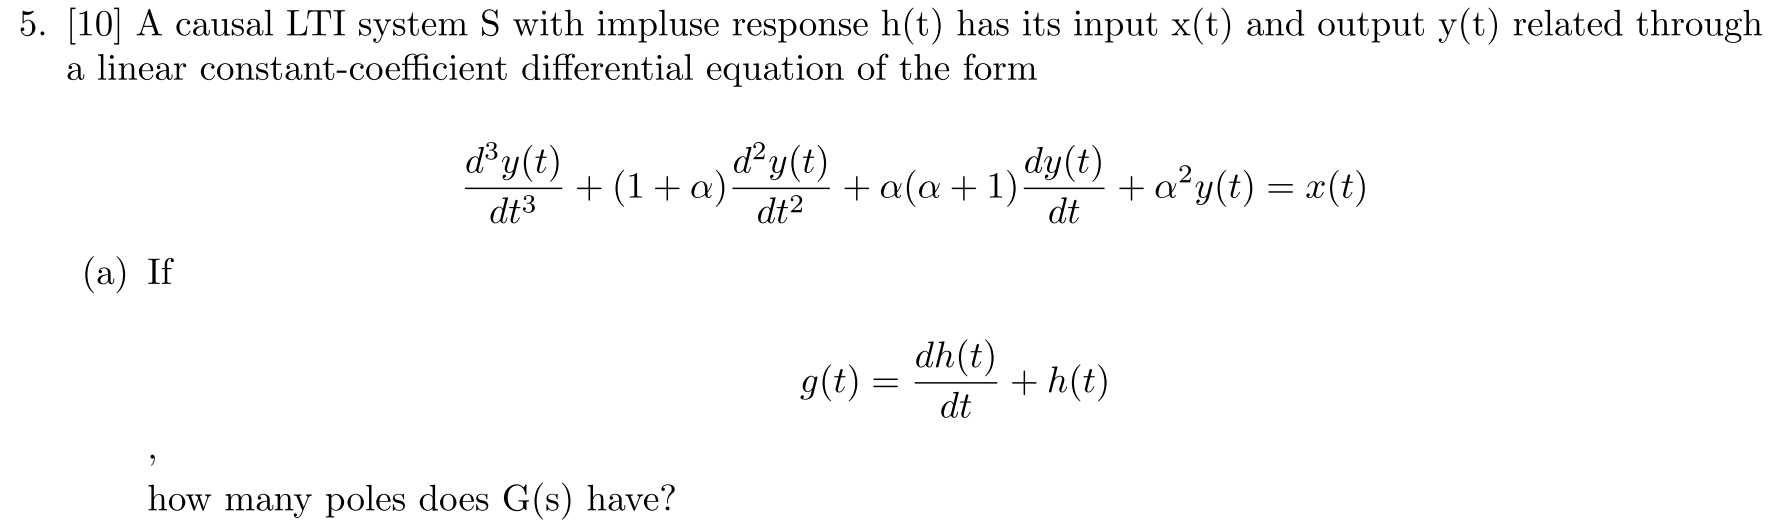
\includegraphics[width=1\linewidth]{q5}
    \end{figure}
    Hint: use long division
\end{frame}

\begin{frame}[t]
    \frametitle{Exercise: HW6 Q7}
    \begin{figure}
        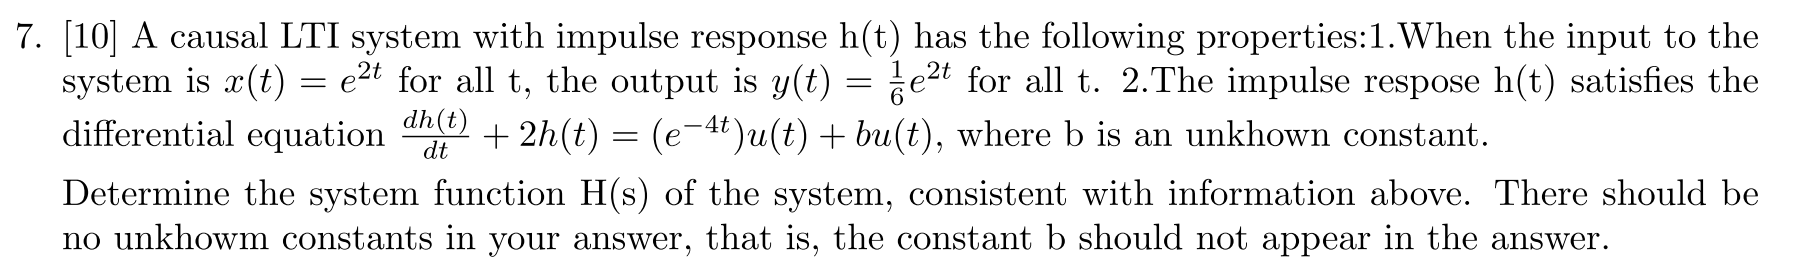
\includegraphics[width=1\linewidth]{q7}
    \end{figure}
    Hint: when input is an exponential signal
\end{frame}



\begin{frame}
    \frametitle{Conclusion - for Chap. 9}
    \begin{itemize}
    \item FS vs. FT vs. LT
    \item Focus on system prospective
    \item Practice on PFE, block diagram, etc 
    \end{itemize}
\end{frame}

%-------------------------------------------------




\section{Conclusion}
\begin{frame}
\frametitle{Conclusion - for the course}
\begin{itemize}
\item LTI system, impulse response, convolution - Foundation, Time domain
\item Fourier Analysis - signal, system
\item Filtering, Sampling, Communication - most interesting topics to me
\item Laplace Transform - ROC, system, block diagram
\item This course is one of the most inspiring course I have ever took, as it provides a sense of the strong connection between mathematics and the real world.
\item And I join research group then.
\item If you are interested in signal processing, consider taking: VE351; VE401, VE501; VE455, VE489; VV214/417
\end{itemize}
\end{frame}

%------------------------------------------------

\begin{frame}
\Huge{\centerline{The End}}
\end{frame}

%----------------------------------------------------------------------------------------

\end{document} 